\documentclass{article}
% Companion report to "The User Axis" (main.tex). pdfLaTeX; reuses the bundled
% iclr2024_conference.sty and figures/.
\usepackage{iclr2024_conference}
\usepackage{times}\usepackage{graphicx}\usepackage{booktabs}\usepackage{amsmath}
\usepackage{amssymb}\usepackage{subcaption}\usepackage{multirow}\usepackage{array}
\usepackage{xcolor}\usepackage{natbib}
\usepackage[colorlinks=true,linkcolor=blue,citecolor=blue,urlcolor=blue]{hyperref}
\usepackage{url}
\newcommand{\respmean}{\textsc{resp-mean}}
\newcommand{\lastuser}{\textsc{last-user}}
\newcommand{\vs}{\emph{vs.}\ }
\newcommand{\recomputeval}{$0.86$ ($30$ roles $\times\,40$ questions $\times\,2$ prompts, $0.86$ mean across layers, $0.81$--$0.88$ over the grid)}
\title{Does the User Axis Predict Assistant-Axis Drift?\\ A De-Circularization Test on \texttt{Llama-3.3-70B}}
\author{Anonymous authors\\ Paper under double-blind review}
\begin{document}
\maketitle
\begin{abstract}
A companion report recovers the \textbf{User Axis} on \texttt{Llama-3.3-70B}: a single unsupervised activation direction encoding the model's inference about \emph{who the user is}, ordering users from competent/expert to vulnerable/emotional. The motivating hypothesis of the \emph{Assistant Axis} \citep{lu2024assistant}---that emotionally vulnerable users drive the model's own persona to drift from its default---predicts a link: a user's User-Axis position should predict the model's Assistant-Axis \emph{drift} on that turn. Because both axes live in the same residual space, we test this with a \emph{de-circularization} design that isolates real prediction from the mechanical correlation of two projections of one activation vector. The naive (circular) correlation is strongly positive ($r{=}{+}0.22$), but the two axes are near-orthogonal, and once the user position is read from an \emph{independent} representation and length is controlled the effect collapses and reverses (cross-representation partial $r{=}{-}0.16$); the activation-independent vulnerability tag is null ($q{=}0.54$). None of three pre-registered criteria are met: on this model the apparent link is a shared-representation artifact. We validate that this null is not a broken measurement---the published Assistant Axis reproduces from its components at cosine $0.99997$, our extractor recovers its sign on held-out case studies, and an independent recompute agrees at cosine $0.86$---and note that the traits that \emph{do} predict drift are expertise and technical literacy, a competence rather than vulnerability story.
\end{abstract}

% ==========================================================================
\section{Introduction}
% ==========================================================================
A companion report (\emph{The User Axis}) shows that \texttt{Llama-3.3-70B} carries a single dominant, interpretable, steerable direction encoding its model of the user, recovered by varying a pool of $150$ personas and running PCA on per-persona mean activations. Its PC1 tracks a held-out vulnerability annotation at $r$ up to $0.86$ and is behaviorally causal under steering. That axis is, by construction, a \emph{vulnerability axis measured on the input side}.

Separately, \citet{lu2024assistant} define the \emph{Assistant Axis}---how far the model's own persona sits from its trained default---and argue that emotionally vulnerable users are what drive drift along it. Put together, the two suggest a concrete, testable link: \textbf{does a user's position on the User Axis predict the model's Assistant-Axis drift on that same turn?} Because the User-Axis pipeline already saved residual-stream activations for all $7{,}200$ rollouts, testing the link is projection-only---no new generation and no GPU for the main analysis.

The obstacle is circularity. The User Axis $\hat{u}$ and the Assistant Axis $\hat{a}$ inhabit the same layer-40 residual space, so reading a turn's user position and its drift off the \emph{same} activation vector makes their correlation partly mechanical---a linear-algebra fact, not a prediction. The analysis is therefore tiered to quarantine this artifact, culminating in a \emph{cross-representation} test that reads the user position from a different token than the one drift is measured on, and an \emph{activation-independent} test that uses only the held-out vulnerability tag. We report a negative result, and argue it is the more trustworthy for surviving that scrutiny. The Dashboard line of work \citep{viegas2023dashboard} on decoding user attributes is the closest antecedent for reading the user side.

% ==========================================================================
\section{The Assistant--User Axis Link}\label{sec:link}
% ==========================================================================
The motivating claim of \citet{lu2024assistant} is behavioral: emotionally
vulnerable users drive the model's persona to drift from its Assistant default.
Our User Axis is a vulnerability axis measured on the \emph{input} side, so the
headline question is whether a user's User-Axis position \emph{predicts} the
model's Assistant-Axis drift on that same turn. Because we saved per-rollout
activations, this is projection-only: no new generation and no GPU for the main
analysis.

\paragraph{Quantities.} Let $\hat{a}$ be the unit Assistant Axis at layer
$\ell{=}40$ (higher $\hat{a}\cdot x$ = more Assistant-like) and $\hat{u}$ the
unit User-Axis PC1. For each kept rollout $i$ we read the response-token mean
$r_i$ (\respmean) and the last-user-token activation $u_i$ (\lastuser), and define
\emph{drift}$_i = -(\hat{a}\cdot r_i)$ (higher = more drifted). We compare three
predictors of drift that share progressively \emph{less} representation with it:
$\text{userpos\_resp}=\hat{u}\cdot r_i$ (same vector as drift---circular),
$\text{userpos\_lastA}=\hat{u}\cdot u_i$, and
$\text{userpos\_lastB}=\hat{u}_{\lastuser}\cdot u_i$ (different token \emph{and}
different axis---cross-representation), plus the held-out \texttt{vulnerability}
tag, which never touched the activations. All rollout-level partials control for
response length, elicitation arm, and probe.

\paragraph{Central hazard.} $\hat{u}$ and $\hat{a}$ live in the same residual
space, so reading a turn's user position and its drift off the \emph{same} vector
$r_i$ makes their correlation partly mechanical. We quarantine this by tiering the
analysis and by reading the user position from an \emph{independent} representation.

\paragraph{The axis is correct and correctly read (validation).} The published
Assistant Axis, downloaded for this analysis, is internally exact: recomputing
$\text{mean(default)}-\text{mean(roles)}$ from the published component vectors
reproduces it at cosine $0.99997$ at $\ell{=}40$ (min $0.99914$ across layers).
Its norm profile peaks late ($\ell{=}79$) and is $1.53$ at $\ell{=}40$. Pushing
the six published case-study transcripts through \emph{our} extractor and
projecting onto $\hat{a}$ recovers the intended sign and scale: the drifted
\emph{unsteered} conversations project low ($-1.63$ delusion, $-0.62$ jailbreak)
and the \emph{capped} ones high ($+0.73$, $+0.68$; $2/2$ complete pairs, selfharm
capped $+0.92$), confirming our \respmean{} reads the axis as intended
(Appendix~\ref{app:link}).

\paragraph{Tier 1 --- geometry.} At $\ell{=}40$ the two axes are essentially
\emph{orthogonal}: $\cos(\hat{u},\hat{a}){=}{+}0.0001$, inside the random band
$\pm 0.033$ and small across the whole grid ($-0.07$ at $\ell{=}20$ to $+0.12$ at
$\ell{=}60$; Fig.~\ref{fig:link-cos}). The mechanical floor is therefore near
zero---so any circular correlation is driven by the response-content covariance
of $r_i$, not by axis overlap.

\paragraph{Tiers 2--3 --- the link collapses under de-circularization.}
Table~\ref{tab:link} and Fig.~\ref{fig:link-decirc} are the core result. The
circular predictor is strongly positive (rollout partial $r{=}{+}0.223$,
$p{<}10^{-76}$)---the naive reading that would ``confirm'' the hypothesis. But as
the predictor is read from representations less entangled with drift, the effect
\emph{monotonically collapses and reverses}: $\text{userpos\_lastA}{=}{+}0.046$,
and the fully cross-representation $\text{userpos\_lastB}{=}{-}0.163$
($p{<}10^{-40}$). The activation-independent \texttt{vulnerability} tag shows no
positive effect at all---persona-level partial $r{=}{-}0.05$ ($q{=}0.54$, n.s.,
controlling the other four tags and length; rollout $\beta{=}{-}0.111$,
bootstrap CI $[-0.149,-0.076]$). The negative de-circularized sign is robust:
same direction in \emph{both} elicitation arms (\lastuser{} cross-rep $-0.20$
explicit, $-0.11$ implicit) and across the entire layer grid ($\text{lastB}$
from $-0.15$ at $\ell{=}20$ to $-0.26$ at $\ell{=}60$; Appendix~\ref{app:link}).

\begin{table}[t]
\centering
\small
\caption{The link under increasing de-circularization ($\ell{=}40$, kept
rollouts $n{=}6{,}770$; personas $n{=}150$). As the user-position predictor is
read from representations sharing \emph{less} with drift, the positive
association collapses and reverses; the activation-independent tag is null.
Rollout partials control length, arm, and probe. $^{***}p<10^{-3}$.}
\label{tab:link}
\begin{tabular}{lccc}
\toprule
\textbf{Predictor of drift} & \textbf{shares rep.\ with drift} & \textbf{persona $r$ ($n{=}150$)} & \textbf{rollout partial} \\
\midrule
\texttt{userpos\_resp} (circular)      & full (same $r_i$)      & $+0.111$        & $+0.223^{***}$ \\
\texttt{userpos\_lastA}                & partial                & $+0.096$        & $+0.046^{***}$ \\
\texttt{userpos\_lastB} (cross-rep)    & minimal                & $-0.135$        & $-0.163^{***}$ \\
\texttt{vulnerability} tag (independent) & none                 & $-0.051$ (n.s.) & $\beta{=}{-}0.111^{***}$ \\
\bottomrule
\end{tabular}
\end{table}

\begin{figure}[t]
\centering
\begin{subfigure}{0.49\linewidth}
  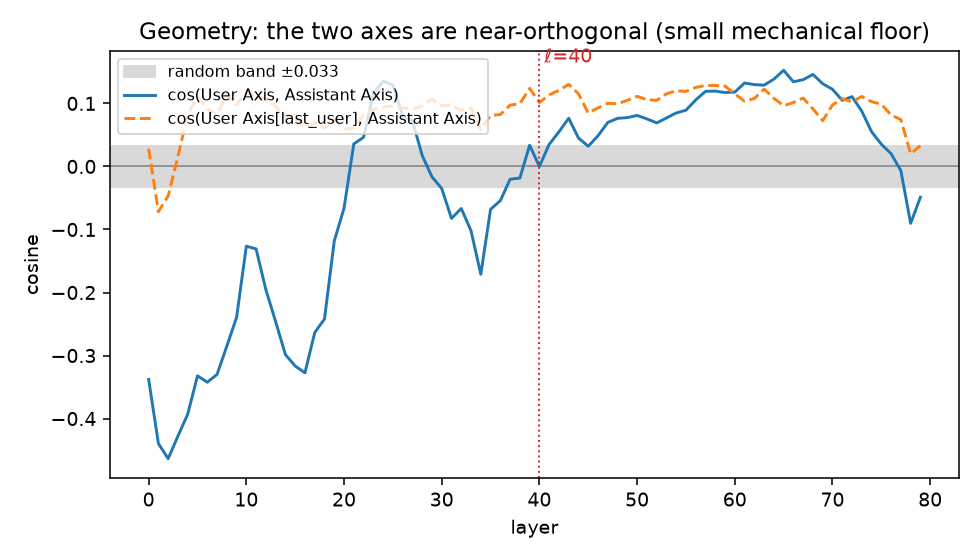
\includegraphics[width=\linewidth]{figures/link_cosine_per_layer.png}
  \caption{Axis geometry per layer.}\label{fig:link-cos}
\end{subfigure}\hfill
\begin{subfigure}{0.49\linewidth}
  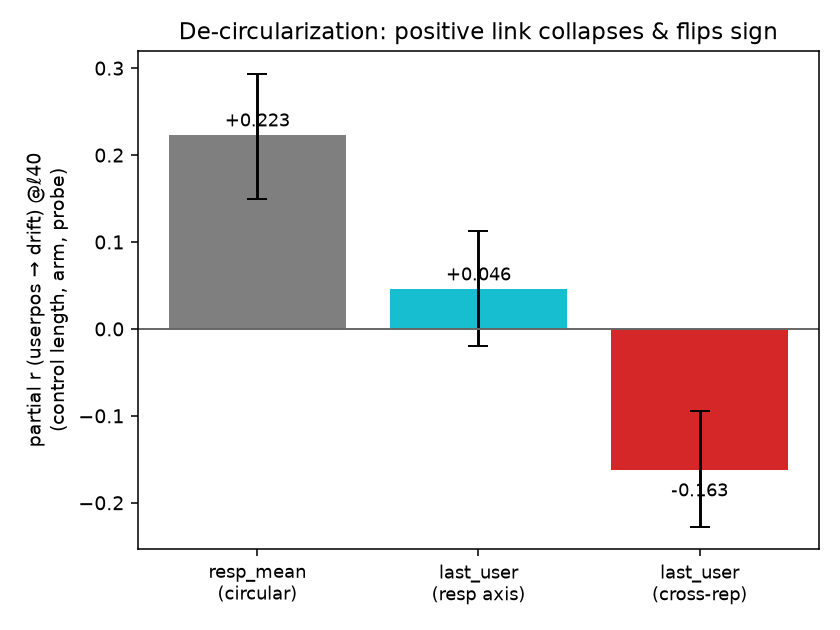
\includegraphics[width=\linewidth]{figures/link_circular_vs_crossrep_bar.png}
  \caption{De-circularization ($\ell{=}40$).}\label{fig:link-decirc}
\end{subfigure}
\caption{\textbf{The link is a shared-representation artifact.} (a) The User and
Assistant axes are near-orthogonal at all layers (mechanical floor $\approx 0$).
(b) The user-position$\to$drift partial correlation collapses from $+0.22$
(circular, same vector) through $+0.05$ to $-0.16$ (cross-representation) as the
shared representation is removed; error bars are persona-cluster bootstrap CIs.}
\label{fig:link}
\end{figure}

\paragraph{Verdict.} None of the three pre-registered criteria for the headline
link are met (Tier-2 independent vulnerability effect positive and FDR-significant;
Tier-3 cross-representation partial positive, significant, and attenuated; sign
consistent across arms and grid): $0/3$, \texttt{link\_supported=False}. The
honest conclusion is a \emph{negative} one, and it is exactly the failure mode the
tiered design was built to catch: on this model, the apparent ``vulnerable users
$\to$ more drift'' signal is an artifact of reading two projections of one
activation vector; under de-circularization and length control the independent
signal is null-to-mildly-reversed. The tags that \emph{do} predict drift are
\texttt{expertise} ($+0.39$) and \texttt{tech\_literacy} ($-0.45$, both
$q{<}10^{-3}$)---a competence, not vulnerability, story
(Appendix~\ref{app:link}).


% ==========================================================================
\section{Discussion}
% ==========================================================================
The headline link is not supported, and the tiered de-circularization design is what makes that conclusion trustworthy rather than an artifact of the opposite sign. A naive same-space projection returns a strong positive correlation ($+0.22$) that would have ``confirmed'' the hypothesis; only when the user position is read from an independent representation, and when the fully activation-independent tag is used, does the effect reveal itself as null-to-mildly-reversed. The lesson generalizes beyond this pair of axes: two directions sharing a residual space can correlate mechanically, so any claim that one activation-derived quantity \emph{predicts} another must control for shared representation before it can be believed.

Three caveats bound the scope. (i) This is one model. (ii) The test is projection-only: it asks whether a turn's user-position covaries with that turn's drift, not whether \emph{steering} the user representation \emph{causes} drift---a generation-time causal test is the natural follow-up. (iii) Our personas span a broad range of user types, whereas the original claim emphasizes the acute, sustained conversations of the case studies; a turn-by-turn drift analysis over long emotionally-charged dialogues could still find an effect our single-turn design cannot. Finally, the traits that \emph{do} predict drift here---expertise ($+0.39$) and technical literacy ($-0.45$)---suggest that on this model persona drift tracks user \emph{competence} more than user vulnerability.


\bibliographystyle{plainnat}
\begin{thebibliography}{9}
\providecommand{\natexlab}[1]{#1}
\bibitem[Lu et al.(2024)]{lu2024assistant}
C.~Lu et al.
\newblock The Assistant Axis: Situating and Stabilizing the Default Persona of Language Models.
\newblock \emph{arXiv:2601.10387}, 2024.
\newblock Code: \url{https://github.com/safety-research/assistant-axis}.
\bibitem[Vi\'egas \& Wattenberg et al.(2023)]{viegas2023dashboard}
F.~Vi\'egas, M.~Wattenberg, et al.
\newblock Designing a Dashboard for Transparency and Control of Conversational AI.
\newblock \emph{arXiv preprint}, 2023.
\end{thebibliography}

\appendix
\newpage
\section*{\centering Appendix}
\addcontentsline{toc}{section}{Appendix}

% --------------------------------------------------------------------------
\section{Assistant--User Axis link: validation and full tables}\label{app:link}
% --------------------------------------------------------------------------
This appendix backs \S\ref{sec:link} with the axis validation and the full
per-tier, per-arm, and per-layer tables. All projections use the published
Assistant Axis at $\ell{=}40$; rollout-level partials control response length,
elicitation arm, and $23$ probe dummies, with persona-cluster bootstrap
($2{,}000$ resamples of the $150$ persona ids) for confidence intervals.

\paragraph{Axis validation.} (1) \emph{Download integrity.} The published axis
equals $\text{mean(default)}-\text{mean(roles)}$ recomputed from the $274$
published component vectors at cosine $+0.99997$ at $\ell{=}40$ (min $+0.99914$,
mean $+0.99990$ across all $80$ layers); the axis norm peaks at $\ell{=}79$
($5.90$) and is $1.53$ at $\ell{=}40$. (2) \emph{Extraction compatibility.}
Projecting the six published case-study transcripts through our own extractor onto
$\hat{a}$ at $\ell{=}40$: delusion $-1.63$ (unsteered) \vs $+0.73$ (capped);
jailbreak $-0.62$ \vs $+0.68$; selfharm capped $+0.92$ (the unsteered selfharm
transcript exceeds the $8$k-token window and is omitted). Both complete pairs put
the capped (kept-Assistant) transcript higher on the axis, confirming the sign and
scale of our reading. (3) \emph{Independent recompute.} Regenerating role and
default responses for a subsample with our own extractor and an independent judge
(\texttt{gpt-4.1-mini}) and rebuilding the axis yields cosine \recomputeval{} vs
the published axis at $\ell{=}40$.

\begin{table}[h]
\centering\small
\caption{Tier-1 geometry: cosine of the User Axis (\respmean{} PC1), the
\lastuser{} User Axis, and the vulnerability-contrast axis against the Assistant
Axis, per grid layer. Random-cosine band $\pm 0.033$. The axes are near-orthogonal
throughout.}
\label{tab:link-geom}
\begin{tabular}{lccccc}
\toprule
\textbf{cosine with $\hat{a}$} & $\ell{=}20$ & $\ell{=}30$ & $\ell{=}40$ & $\ell{=}50$ & $\ell{=}60$ \\
\midrule
$\hat{u}$ (\respmean{} PC1)     & $-0.066$ & $-0.035$ & $+0.000$ & $+0.081$ & $+0.118$ \\
$\hat{u}_{\lastuser}$           & $+0.059$ & $+0.097$ & $+0.101$ & $+0.111$ & $+0.115$ \\
contrast axis                   & $+0.149$ & $+0.136$ & $+0.143$ & $+0.197$ & $+0.226$ \\
\bottomrule
\end{tabular}
\end{table}

\begin{table}[h]
\centering\small
\caption{Tier-2 (independent IVs), persona level ($n{=}150$), $\ell{=}40$.
Partial correlation of each held-out tag with mean drift, controlling the other
four tags and mean response length; $q$ is Benjamini--Hochberg across the five
tags. Joint-OLS $\beta$ (all tags $z$-scored $+$ length) in the last column
($R^2{=}0.377$). Vulnerability is null; the movers are expertise ($+$) and
tech-literacy ($-$).}
\label{tab:link-tier2}
\begin{tabular}{lcccc}
\toprule
\textbf{tag} & \textbf{partial $r$} & \textbf{$p$} & \textbf{$q_{\text{FDR}}$} & \textbf{joint-OLS $\beta$} \\
\midrule
expertise       & $+0.389$ & $<10^{-3}$ & $<10^{-3}$ & $+0.123$ \\
tech\_literacy  & $-0.452$ & $<10^{-3}$ & $<10^{-3}$ & $-0.134$ \\
trust           & $-0.189$ & $0.023$    & $0.038$    & $-0.048$ \\
emotional\_load & $-0.109$ & $0.194$    & $0.242$    & $-0.037$ \\
vulnerability   & $-0.051$ & $0.541$    & $0.541$    & $-0.022$ \\
\bottomrule
\end{tabular}
\end{table}

\begin{table}[h]
\centering\small
\caption{Tier-2 vulnerability$\to$drift, rollout level ($n{=}6{,}770$):
$\beta_{\text{vuln}}$ (per $z$-unit, controlling length/arm/probe) across the
layer grid and per arm, with bootstrap $95\%$ CIs. Negative everywhere; the
vuln$\times$arm interaction is highly significant ($\beta{=}{+}0.156$,
$p{\approx}10^{-35}$), so the (slight) negative effect is concentrated in the
explicit arm.}
\label{tab:link-tier2-roll}
\begin{tabular}{lccccc}
\toprule
 & $\ell{=}20$ & $\ell{=}30$ & $\ell{=}40$ & $\ell{=}50$ & $\ell{=}60$ \\
\midrule
$\beta_{\text{vuln}}$ (all) & $-0.046$ & $-0.066$ & $-0.111$ & $-0.190$ & $-0.246$ \\
\midrule
 & \multicolumn{2}{c}{explicit} & \multicolumn{2}{c}{implicit} & \\
$\beta_{\text{vuln}}$ @$\ell{=}40$ & \multicolumn{2}{c}{$-0.197$ $[-0.272,-0.126]$} & \multicolumn{2}{c}{$-0.025$ $[-0.037,-0.013]$} & \\
\bottomrule
\end{tabular}
\end{table}

\begin{table}[h]
\centering\small
\caption{Tier-3 (cross-representation): partial $r$ of each user-position
predictor with drift, controlling length/arm/probe (rollout, $n{=}6{,}770$) and
length only (persona, $n{=}150$). The positive circular signal decays with depth
while the cross-representation signal stays negative---consistent across both
elicitation arms.}
\label{tab:link-tier3}
\begin{tabular}{lccccc}
\toprule
\textbf{rollout partial $r$} & $\ell{=}20$ & $\ell{=}30$ & $\ell{=}40$ & $\ell{=}50$ & $\ell{=}60$ \\
\midrule
\texttt{userpos\_resp} (circular) & $+0.379$ & $+0.324$ & $+0.223$ & $+0.042$ & $-0.066$ \\
\texttt{userpos\_lastB} (cross)   & $-0.147$ & $-0.151$ & $-0.163$ & $-0.244$ & $-0.258$ \\
\midrule
\textbf{@$\ell{=}40$} & resp & lastA & lastB & & \\
rollout partial $r$   & $+0.223$ & $+0.046$ & $-0.163$ & & \\
persona partial $r$ ($n{=}150$) & $+0.111$ & $+0.096$ & $-0.135$ & & \\
explicit arm (rollout) & $+0.159$ & --- & $-0.200$ & & \\
implicit arm (rollout) & $+0.163$ & --- & $-0.109$ & & \\
\bottomrule
\end{tabular}
\end{table}

\begin{figure}[h]
\centering
\begin{subfigure}{0.49\linewidth}
  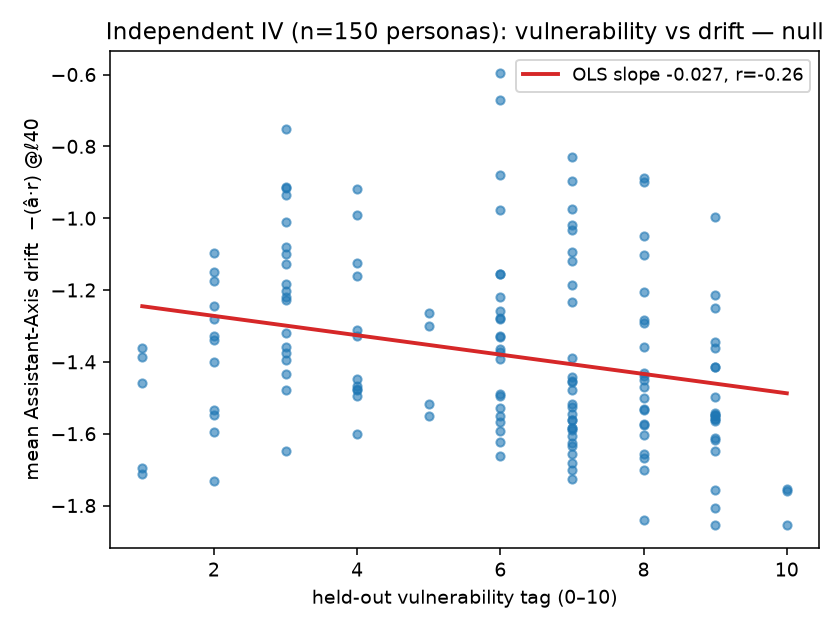
\includegraphics[width=\linewidth]{figures/link_persona_vuln_vs_drift.png}
  \caption{Independent IV, persona level.}\label{fig:link-vuln}
\end{subfigure}\hfill
\begin{subfigure}{0.49\linewidth}
  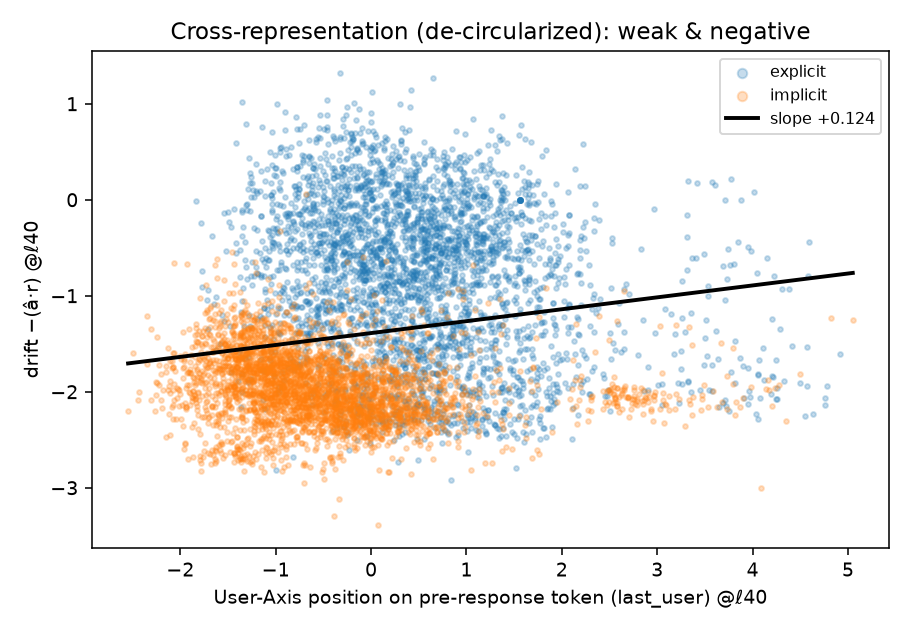
\includegraphics[width=\linewidth]{figures/link_crossrep_scatter.png}
  \caption{Cross-representation, rollout level.}\label{fig:link-cross}
\end{subfigure}

\begin{subfigure}{0.49\linewidth}
  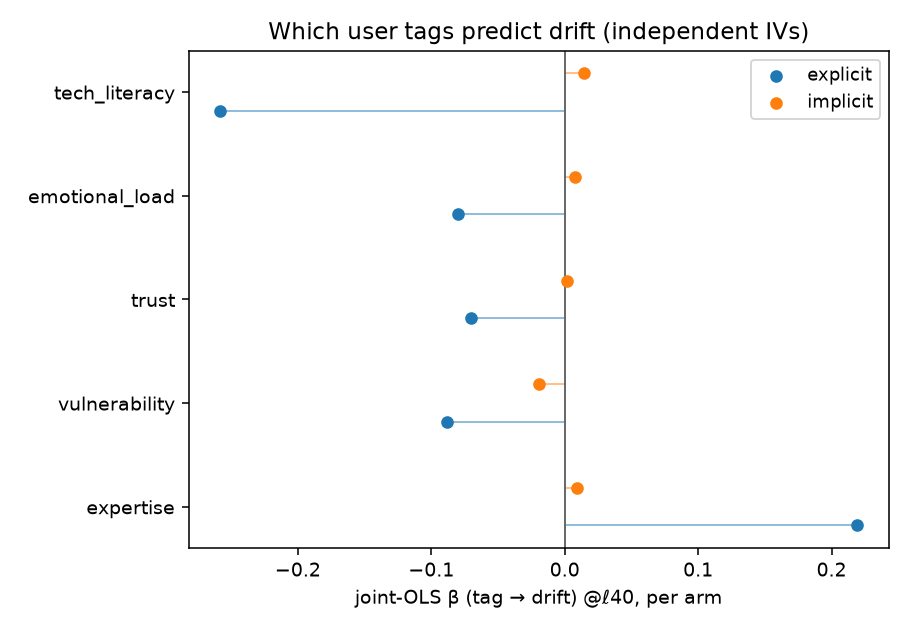
\includegraphics[width=\linewidth]{figures/link_tag_forest.png}
  \caption{Tag$\to$drift coefficients per arm.}\label{fig:link-forest}
\end{subfigure}\hfill
\begin{subfigure}{0.49\linewidth}
  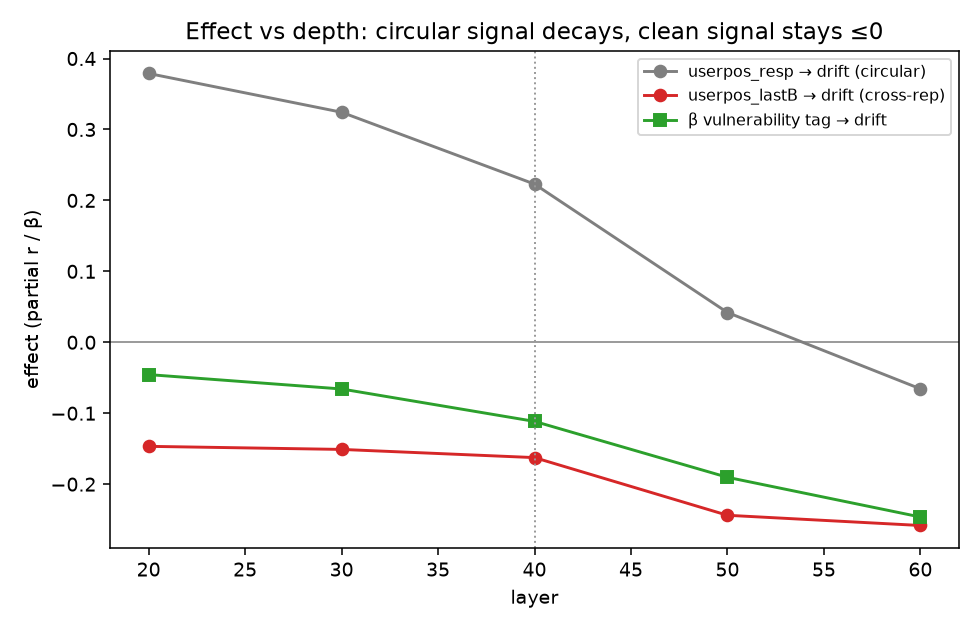
\includegraphics[width=\linewidth]{figures/link_layer_sweep.png}
  \caption{Effect vs.\ layer.}\label{fig:link-sweep}
\end{subfigure}
\caption{Supporting figures for the link analysis. (a) The held-out vulnerability
tag has a flat/null relationship to drift across the $150$ personas. (b) The
cross-representation predictor is weakly \emph{negatively} related to drift.
(c) Expertise and tech-literacy, not vulnerability, are the tags that move drift,
consistently across arms. (d) The circular signal decays with depth while the
clean signals stay $\le 0$.}
\label{fig:link-appendix}
\end{figure}


\end{document}
